\subsubsection{Operationsverstärker} % (fold)
\label{ssub:Operationsverstärker}

\begin{frame}
    \frametitle{Operationsverstärker}
    \framesubtitle{}
    \begin{columns}[c]
    \column{0.6\textwidth}
    \begin{block}{}
        \begin{itemize}
            \item Variables Bauteil für verschiedene Schaltungen
            \item Aufbau:
                \begin{itemize}
                    \item invertierender Eingang
                    \item nichtinvertierender Eingang
                    \item Ausgang
                    \item Versorgungseingänge
                \end{itemize}
            \item Eigenschaften (ideal):
                \begin{itemize}
                    \item unendlich große Gegentaktverstärkung
                    \item perfekte Gleichtaktunterdrückung 
                    \item unendliche Verstärkung
                \end{itemize}
        \end{itemize}
    \end{block}
    \column{0.4\textwidth}
    \begin{figure}[H]
    \begin{center}
            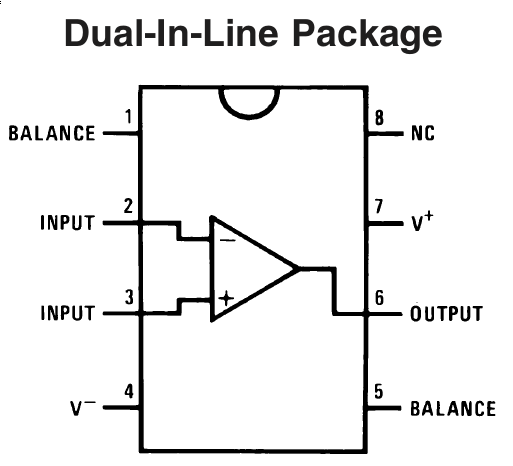
\includegraphics[scale=0.2]{./img/misc/opv_pins.png}
    \end{center}
    \end{figure}
    \begin{figure}[H]
    \begin{center}
            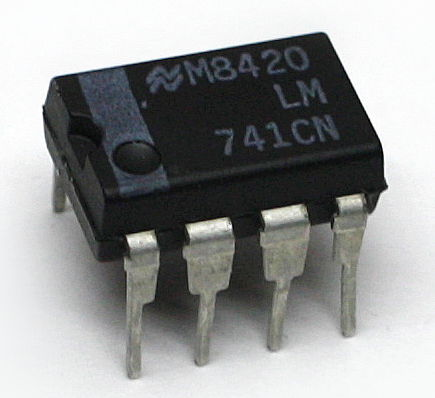
\includegraphics[scale=0.2]{./img/misc/opv_photo.png}
    \end{center}
    \end{figure}
    \end{columns}    
\end{frame}

\begin{frame}
    \frametitle{Operationsverstärker}
    \framesubtitle{}
    \begin{columns}[c]  
        \column{0.6\textwidth}
        \begin{block}{Goldene Regeln:}
             \begin{enumerate}
                 \item Der Ausgang wird stets Versuchen eine Spannung
                 auszugeben so dass die Differenz der Eingansspannung 0 ist:
                 \begin{equation*}
                     \Delta U = U_+ - U_- = 0
                 \end{equation*}
                 \item In die Eingänge $+$ und $-$ fließt kein Strom:
                 \begin{equation*}
                     I_+ = I_- = 0
                 \end{equation*}
             \end{enumerate}
        \end{block}
        \column{0.4\textwidth}
        \begin{figure}[H]
        \begin{center}
                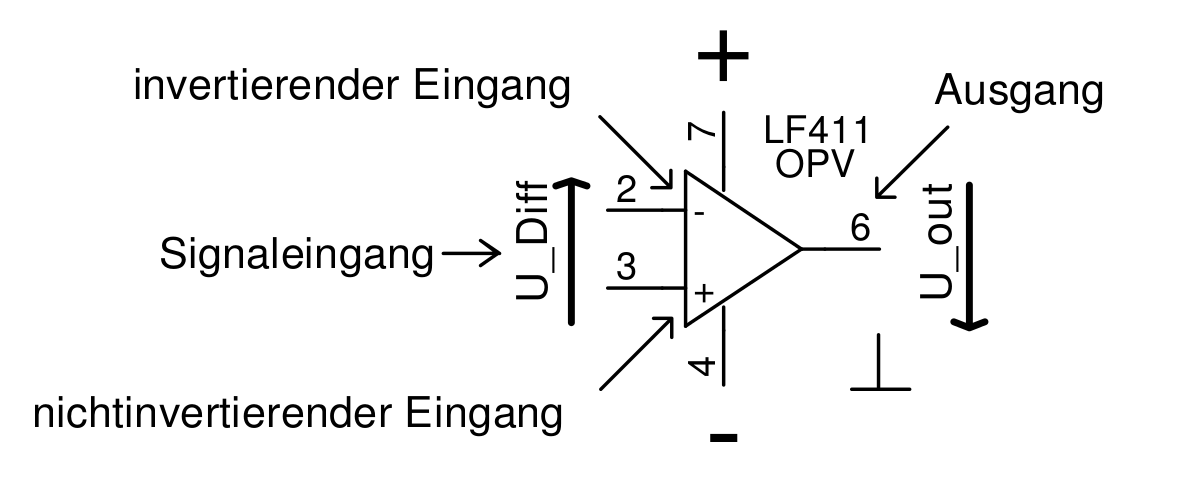
\includegraphics[scale=0.2]{./img/misc/opv_schaltung.png}
        \end{center}
        \end{figure}
    \end{columns}
\end{frame}

% subsubsection Operationsverstärker (end)
